\section{Test Platform}
\subsection{Hardware}
To test point-to-point transmissions, two identical platforms that could send and receive \ac{lora} transmissions were required. The basis of the designed test platform was HopeRF's\footnote{HopeRF Microelectronics Co. Ltd, China, https://www.hoperf.com/} RFM95W - a packet radio containing a \ac{lora} transceiver design licensed from Semtech; specifically, Adafruit's\footnote{Adafruit, USA, https://www.adafruit.com/} broken out version was used. As a raw packet radio, unlike the popular Microchip RN2483, it provided direct access to the radio interface. An omni-directional 3dBi 868MHz whip antenna was connected to the radio using a soldered uFL connector and a SMA to uFL connector. It was controlled by a Teensy\footnote{Teensy, https://www.pjrc.com/teensy/} 3.6 micro-controller, which also handled all logging responsibilities. A simple breakout circuit was designed and implemented on strip-board to connect the components in a condensed package. Each breakout board featured: a JST-PH2 battery connector, a coin cell holder for the Teensy's real-time-clock (\ac{rtc}), a power switch, a two-mode software switch, and three status LEDs. The schematic can be viewed in Figure \ref{fig:datalogger_schematic}. This was packaged to fit in an IP67 rated container with an internal 1800mAh \ac{lipo} battery. Switches and SMA antenna connectors were external; these were IP67 rated and extra sealing has been added where appropriate. The final dataloggers can be seen in Figure \ref{fig:dataloggers}. The Teensy is equipped with an SD card for storage but, due to cost considerations, a GPS module could not be implemented. The full breakdown of materials can be seen in Figure \ref{fig:datalogger_cost}.

\subsection{Software}
The system was designed such that one device (a slave) could be left unattended at a fixed location and controlled by a second device (a master); this was achieved using a command control system, as seen in Figure \ref{fig:software_cmd_system}. Two command classes were defined for testing purposes; these are as follows:
\begin{itemize}
	\item {\textbf{\texttt{HB\_CMD}}} : Command to trigger simple heartbeat functionality. When a slave receives this command it sends a heartbeat response (a short packet) on the base operating configuration. If in range, the master device will pick this up and alert the user.
	\item {\textbf{\texttt{TD\_CMD}}} : Command to trigger execution of a test definition (\ac{td}). In principle, the master device requests a set of packets to be sent by the slaves using the \ac{td} configuration; this is the basis of all test functionality. The full control flow is explained in detail in Figure \ref{fig:software_testdef_execution}.
\end{itemize}

%Whether a device was a master or a slave was determined by the board identifier stored in the Teensy EEPROM; this meant the same software could be flashed onto both, reducing the chance of software version inconsistencies.

\begin{figure}[H]
    \centering
    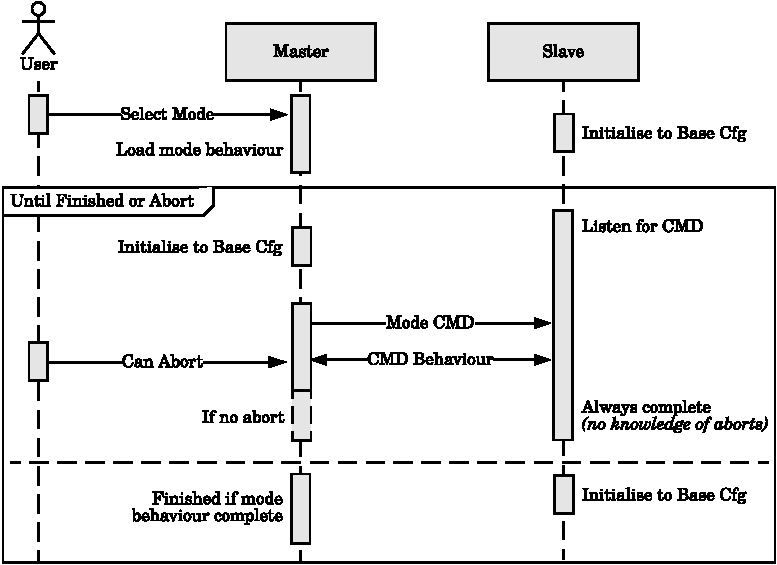
\includegraphics{Figures/software_cmd_system.pdf}
    \caption[Master-Slave command control method]{Diagram showing Master-Slave command control method.}
    \label{fig:software_cmd_system}
\end{figure}

\begin{figure}[H]
    \centering
    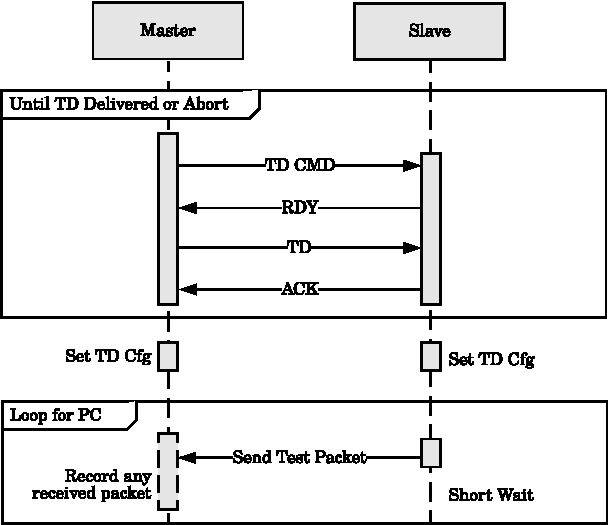
\includegraphics{Figures/software_testdef_execution.pdf}
    \caption[Master-Slave test definition execution method]{Diagram showing test definition execution.}
    \label{fig:software_testdef_execution}
\end{figure}




% the user, could trigger a command to be sent from the master to the receiver. 
%
%Whether a device was a master or a slave was determined by the board identifier stored in the Teensy EEPROM; this meant the same software could be flashed onto both, reducing the chance of software version inconsistencies.
%
% 
%Interfacing with the radio was handled by the RH\_RF95 driver from the Radiohead\footnote{Radiohead, https://www.airspayce.com/mikem/arduino/RadioHead/} library; this meant that only the control logic needed to be implemented. 
%
%
% A high-level overview of the planned test method is visualised in Figure \ref{master_slave_sequence}. \label{datalogger_software}
%
%
%    
%    Initial link testing will make use of two node classes: masters and slaves. The slaves are responsible for sending packets in the configuration requested by the master device. These are in the form of test definitions (TDs) that are stored on the master's memory card and will be processed one at a time. As the proposed system utilises only nodes, slave and master must have the same \ac{sf} and \ac{bw} for receiving the TD. This base state will be hard-coded such that the expected range exceeds or matches that of the longest range TD. The master will expect a certain number of packets (PC) from the slave, those received will have performance figures such as \ac{rssi}, \ac{snr} and \ac{per} recorded to the memory card under the specific test. The slave will wait for a new test definition once the PC has been sent. The master will proceed onto the next TD once the expected test length has expired.